\chapter{Design and implementation}
This chapter will go through the processes of designing and implementing the system for Aalborg Zoo, as well as discussing the thoughts behind the coding and design.

\section{Architectural design}
Upon development of the program, more components, and subsystems have been added to the system structure. The system has been split into smaller parts to get a better understanding of the components of the system, a more detailed class diagram have been made. These components will be discussed in the following section.

\subsection{Component design}
This section will focus on explaining the different components of the program, and their relations. As well as describing the functions of the individual sub-systems, and their components.

\subsubsection{Fields}\todo[Inline]{Better name}
\begin{figure}[H]
    \centering
    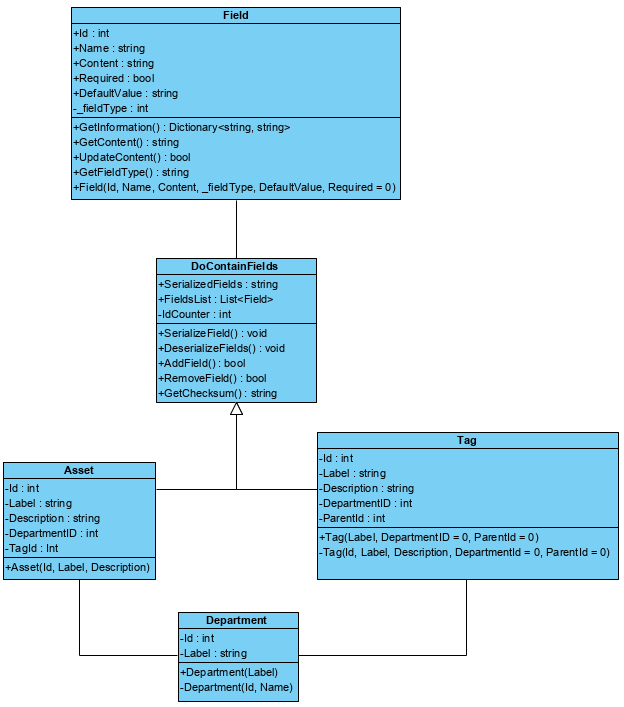
\includegraphics{figures/FieldsComponent.PNG}
    \caption{Componentdiagram for the Field Component}
    \label{fig:FieldsComponent}\todo[Inline]{Upload nyt diagram, med abstrakt DoContainFields}
\end{figure}
This components function is to describe the general in formations needed for the two classes containing instances of \textit{fields}. The classes which needs \textit{fields} are \textit{Asset} and \textit{Tag}, both of these aggregates functions and variables from \textit{DoContainFields}. The functions aggregated are functions related to controlling fields and their behavior on the aggregating classes. As both \textit{Tag} and \textit{Asset} needs to be able to utilize the same functionalities when handling \textit{Fields} and serializing these. 
\par
The serilization of the fields is done to JSON. The reason for choosing to utilize JSON is that MYSQL and other newer database versions, can index JSON so it counts as virtual rows within the database. These virtual rows enables searching the JSON fields, with ordinary SQL queries.



\section{UI design}
Model-View-Viewmodel (MVVM) design pattern